
%\documentclass{elsart}               % The use of LaTeX2e is preferred.

\documentclass[twocolumn]{autart}    % Enable this line and disable the 
                                     % preceding line to obtain a two-column 
                                     % document whose style resembles the
                                     % printed Automatica style.


\usepackage{graphicx}          % Include this line if your 
                               % document contains figures,
%\usepackage[dvips]{epsfig}    % or this line, depending on which
                               % you prefer.

\usepackage{graphicx}
\usepackage[utf8]{inputenc}

%\usepackage[spanish]{babel}
\usepackage{geometry}


\usepackage{ntheorem,lipsum}

\theorembodyfont{\upshape}
\newtheorem{thm}{Teorema}[section]
\newtheorem{definition}{Definition}[section]
\newtheorem{obs}{Observación}[section]
\newtheorem{proposition}{Proposition}[section]
\newtheorem{example}{Ejemplo}[section]
\newtheorem{problem}{Problem}[section]
\newtheorem{hipo}{Hipotesís}[section]

\usepackage{bm}

\usepackage{amsmath}
\usepackage{amssymb}

\DeclareMathOperator*{\argmax}{arg\,max}
\DeclareMathOperator*{\argmin}{arg\,min}
\usepackage{hyperref}
\hypersetup{
    colorlinks=true,
    linkcolor=blue,
    filecolor=magenta,      
    urlcolor=cyan,
}


\numberwithin{equation}{section}


\usepackage[Algoritmo]{algorithm}

\usepackage{algpseudocode}
\usepackage{caption}
\usepackage{subcaption}

\begin{document}

\begin{frontmatter}
\runtitle{Selective Harmonic Elimination via Optimal Control}   % Running title for regular 
                                              % papers but only if the title  
                                              % is over 5 words. Running title 
                                              % is not shown in output.

\title{Multilevel Selective Harmonic Modulation via Optimal Control} % Title, preferably not more 
                                                 % than 10 words.

\thanks[footnoteinfo]{This paper was not presented at any IFAC meeting.}

\author[FD,UD]{Umberto Biccari}\ead{umberto.biccari@deusto.es},    % Add the 
\author[UAM,FD]{Carlos Esteve Yagüe}\ead{carlos.esteve@uam.es},               % e-mail address 
\author[UD]{Jes\'us Oroya}\ead{djoroya@deusto.es}  % (ead) as shown
\address[FD]{Chair of Computational Mathematics, Fundaci\'on Deusto, Avenida de las Universidades 24, 48007 Bilbao, Basque Country, Spain.}  %
\address[UD]{Universidad de Deusto, Avenida de las Universidades 24, 48007 Bilbao, Basque Country, Spain.}  %
\address[UAM]{Departamento de Matem\'aticas, Universidad Aut\'onoma de Madrid, 28049 Madrid, Spain.}  % Please supply                                              
          
\begin{keyword}                           % Five to ten keywords,  
Selective Harmonic Modulation; Optimal Control Theory; Finite-Set Control; Pontryagin's maximum principle; Piece-wise linear penalization.    % chosen from the IFAC 
\end{keyword}                             % keyword list or with the 
                                          % help of the Automatica 
                                          % keyword wizard


\begin{abstract}                          % Abstract of not more than 200 words.
We consider the \emph{Selective Harmonic Modulation}(SHM) problem, consisting in the design of a staircase control signal with some prescribed frequency components. In this work, the SHE problem is addressed as an optimal control one in which the admissible controls are piece-wise constant functions, taking values only in a given finite set. In order to fulfill this constraint, we  introduce a cost functional \UB{with piece-wise linear penalization } which, by means of Pontryagin's maximum principle, makes the optimal control have the desired staircase form. An advantage of our approach, \UB{relevant in practical electrical engineering applications}, is that the number of commutations and the waveform need not be specified a priori. Indeed, our algorithm provides an admissible waveform as well as the location of the switches. Up to the best of our knowledge, this approach to the SHE problem via optimal control is new. Moreover, our methodology may be applicable to other optimal control problems with a finite-set constraint on the control. We also provide several numerical examples in which the SHM problem is solved by using our approach.
\end{abstract}

\end{frontmatter}


\section{Introduction and motivations}\label{Section1}

Selective Harmonic Modulation (SHM) \cite{Rodriguez2002} is a well-known methodology in electrical engineering, employed to improve the performances of a converter by controlling the phase and amplitude of the harmonics in its output voltage. As a matter of fact, this technique allows to increase the power of the converter and, at the same time, to reduce its losses. 

Because of the growing complexity of modern electrical networks, consequence for instance of the high penetration of renewable energy sources, the demand in power of electronic converters is day by day increasing. For this and other reasons, SHM has been a preeminent research interest in the electrical engineering community, and a plethora of SHM-based techniques has been developed in recent years. An incomplete bibliography includes \cite{duranay2017selective,Janabi2020,Yang2017}.

In broad terms, the technique consists in generating a \textit{control signal} with a desired harmonic spectrum by modulating or eliminating some specific lower-order frequencies. In practice, the signal is constructed as a step function with a finite number of switches, taking values only in a given finite set. Such a signal can be fully characterized by two features (see Figure \ref{fig:exampleSHE}): 
\begin{itemize}
	\item[1.] The \textit{waveform}, i.e. the sequence of values that the function takes along the time interval.
	\item[2.] The \textit{switching angles}, i.e. the sequence of times when the signal switches from one value to following one. 
\end{itemize}
Using this simple characterization of the signal, one can reduce, in some situations, the SHM problem to a finite-dimensional optimization problem.
Given a suitable waveform, the SHM problem consists in finding the optimal location of the switching angles. However, this formulation carries some difficulties,  as for instance, the choice of a suitable waveform or the number of switching angles (see Section \ref{sec:SHE_finite-dim_pbm}).  

In this work, we propose a new approach to SHM based on optimal control theory (see Section \ref{sec:Contributions}). The Fourier coefficients in the SHM problem are identified with the terminal state of a controlled dynamical system, where the control is actually the signal, solution to the SHM problem. The main difficulty in our approach arises from the fact that we look for piece-wise constant solutions, taking values only in a given finite set.

This kind of constraint on the control prevents one from applying the classical tools in optimal control theory, such as Pontryagin's maximum principle. In order to bypass this difficulty, we introduce a penalization term for the control, which guarantees that the optimal control will have the desired staircase structure. The optimization is then carried out over the controls in $L^\infty$, and then, standard computational algorithms in optimal control theory can be implemented to solve the SHM problem. The main advantage of our approach is that we do not need to determine a priori the waveform of the solution nor the number of switching angles. Moreover, by choosing different penalization functions for the control, we can obtain solutions to the SHM problem with different waveforms.

\UB{The main contributions of the present paper are as follows:}
\begin{enumerate}
    \item[1.] We reformulate the SHM problem as an optimal control problem with a staircase constraint on the control.
    \item[2.] We introduce a penalization term for the control which implicitly induces the staircase property on the solution. Here we distinguish two cases: when the control set contains only two elements (\UB{bi-level or } bang-bang control) and when it contains more than two elements (multilevel control).
    \item[3.] Our approach allows one to compute solutions to the SHM problem with different waveforms.
    \JO{ 
    \item[4 ] Nuestra aproximación nos permite encontar soluciones de ángulos de conmutación continuas con respecto al target}
    %\item[4.] {\color{red} Continuidad de solucion respecto al target, estimacion superior numero de switches???? }
	% NO te metas alli, que es un verengenal!
\end{enumerate}

{\color{red} Revisar la estructura cuando el paper est\'e terminado.

In this document, we follow the next structure. In the Section \ref{sec:math_formulation}, we introduce a mathematical formulation of a general SHE problem. 
%
In the Section \ref{sec:SHE_finite-dim_pbm}, we show the classical formulation in SHE literature, and we show two main problems because of this aproach. 
%
In the Section \ref{sec:Contributions}, we show our contributions in this problem, where explain the SHE problem as control problem and the strategies to obtain a piece-wise function as optimal control. 
%
In the Section \ref{sec:Simulations} we show a concrete examples solve by control theory. 
%
In the Section \ref{sec:Proof}, we summaries the proof associated to our contribution. 
%
By last, we finished with some conclusion and open problems. 
}

\section{Preliminaries}\label{sec:math_formulation}

This section is devoted to the mathematical formulation of the SHM problem and to the introduction of the notation that will be used throughout the paper. Let 
\begin{align}\label{eq:Udef}
	\mathcal{U} = \{u_1, \ldots, u_L\}
\end{align}
be a given set of $L\geq 2$ real numbers satisfying
\begin{align*}
	u_1 = -1, \; u_L = 1 \;\text{ and } \; u_k<u_{k+1} \quad\; \forall k\in \{1,\ldots, L\}.
\end{align*}
The goal is to construct a step function
\begin{align*}
	u(t):[0,2\pi)\to\mathcal U,
\end{align*}
with a finite number of switches, such that some of its lower-order Fourier coefficients take specific values prescribed a priori.

\begin{figure}[h]
	\centering
	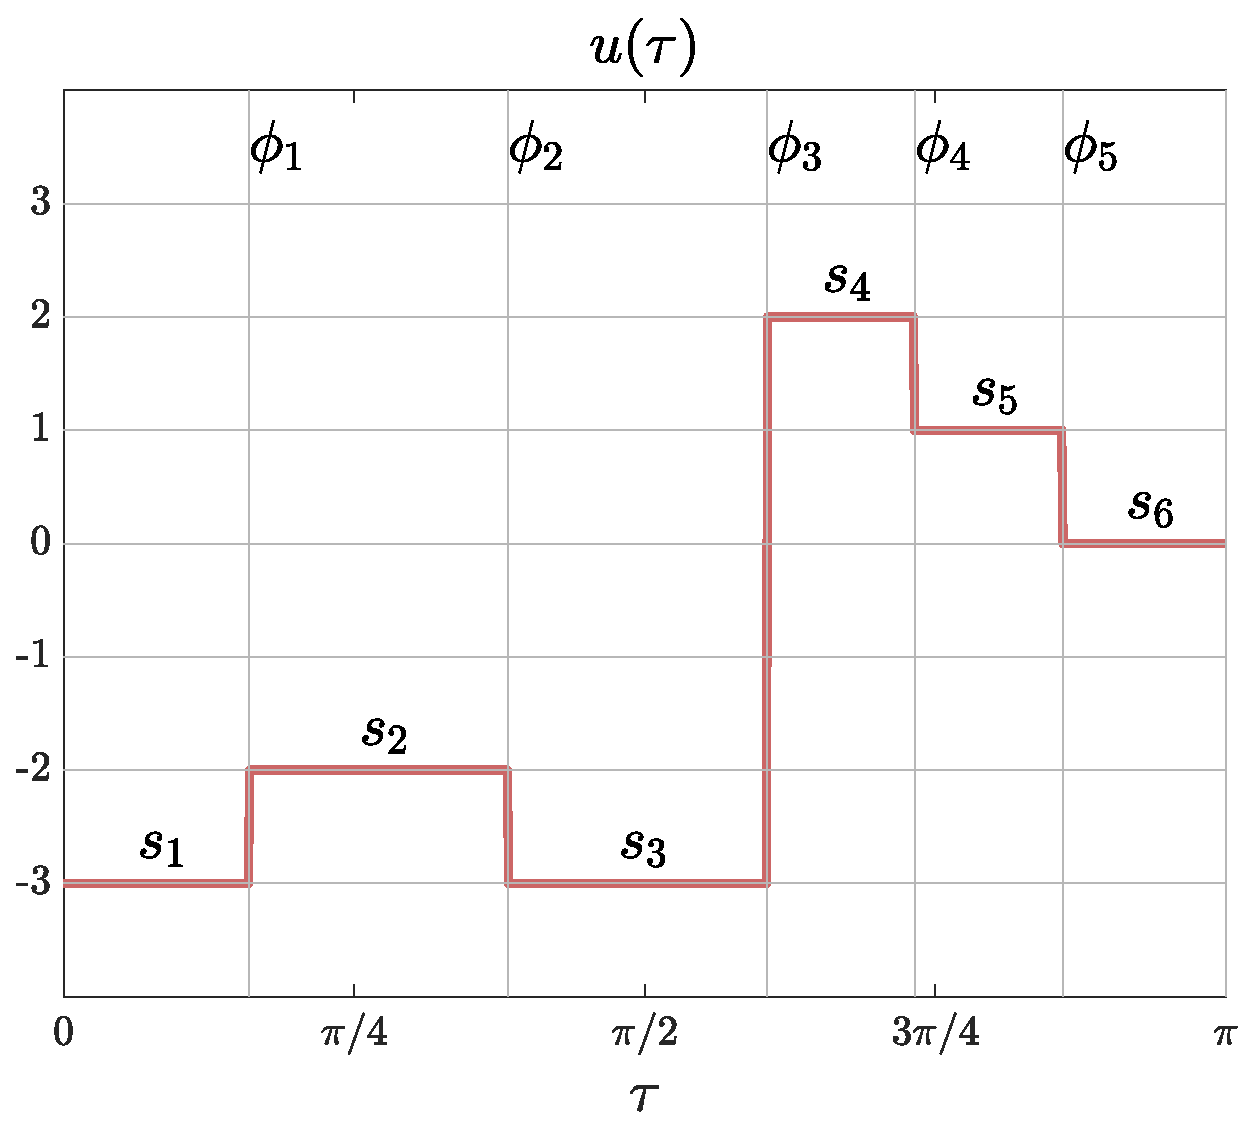
\includegraphics[scale=0.35]{img/fig01.eps} 
	\caption{A possible solution to Problem \ref{pb:SHEp}, where we considered the finite set of control $\mathcal{U} = \{-1, -1/2, 0, 1/2, 1\}$. We show the switching angles $\Phi$ and the waveform $\mathcal{S}$ (see Definition \ref{def: waveform and switching angles}).}
	\label{fig:exampleSHE}
\end{figure}
Due to applications in power converters,  it is typical to only consider functions with \textit{half-wave symmetry}, i.e. satisfying
\begin{align}\label{half-wave symmetry}
	u(t + \pi) = -u(t)\quad \mbox{for all}\; t \in [0,\pi).
\end{align}
In this way, we only need to determine $u$ in the interval $[0,\pi)$. Moreover, as a consequence of this symmetry, the Fourier series of $u$ only involves the odd terms, as the even terms just vanish, i.e.
\begin{align*}
	u(t) = \sum_{\underset{j\, odd}{j \in \mathbb{N}}} a_j \cos(jt)+ \sum_{\underset{j\, odd}{j \in \mathbb{N}}}  b_j \sin(jt),
\end{align*}
where the coefficients $a_j$ and $b_j$ are given by
\begin{equation} \label{eq:an}
	\begin{aligned}
		a_j = \frac{2}{\pi} \int_0^\pi u(\tau ) \cos(j \tau)\,d\tau, 
		\\[5pt]
		b_j = \frac{2}{\pi} \int_0^\pi u(\tau)  \sin(j \tau)\,d\tau.
	\end{aligned}
\end{equation}
In view of the half-wave symmetry \eqref{half-wave symmetry}, in what follows, we will only work with the restriction $u|_{[0,\pi)}$, which, with some abuse of notation, we still denote by $u$. 

As we anticipated,  we are only considering piece-wise constant functions, with a finite number of switches, taking values in $\mathcal{U}$.
More precisely, we look for functions $u: [0,\pi)\to \mathcal{U}$ of the form
\begin{align}\label{eq:uExpl}
	&u (t)= \sum_{m=0}^M s_m\chi_{[\phi_m,\phi_{m+1})} (t)
\end{align}
for some $\mathcal{S} = \{ s_m\}_{m=0}^M$,  with $M\in \mathbb{N}$, satisfying
\begin{align*}
	s_m\in \mathcal{U} \; \text{ and } \; s_m\neq s_{m+1} \quad \forall m\in \{0,\ldots, M\}
\end{align*}
and $\Phi = \{ \phi_m\}_{m=1}^{M}$ satisfying
\begin{align*}
	0= \phi_0 < \phi_1 <\ldots < \phi_M < \phi_{M+1} = \pi .
\end{align*}
In \eqref{eq:uExpl}, $\chi_{[\phi_m,\phi_{m+1})}$ denotes the characteristic function of the interval $[\phi_m,\phi_{m+1})$.

\medskip

\begin{definition}\label{def: waveform and switching angles}
For a function $u: [0,\pi) \to \mathcal{U}$ of the form \eqref{eq:uExpl}, we refer to $\mathcal{S}$ as the \emph{waveform}, and we refer to $\Phi$ as the \emph{switching angles}.
\end{definition}

Observe that any function $u$ of the form \eqref{eq:uExpl} is fully characterized by its waveform $\mathcal{S}$ and its switching angles $\Phi$.
Figure \ref{fig:exampleSHE} shows an example of a function $u$ satisfying \eqref{eq:uExpl}. 

\UB{ 
In the practical engineering applications that motivated our study, due to technical limitations, it is preferable to employ signals taking consecutive values in $\mathcal{U}$. In the sequel, we will refer to this property of the waveform as the \emph{staircase property}.
}
We can rigorously formulate this property as follows: we say that a signal $u$ of the form \eqref{eq:uExpl} satisfies the staircase property if its waveform $\mathcal{S}$ satisfies
\begin{equation}\label{eq:staircase prop}
	(s_m,s_{m+1}) \cap \mathcal{U} = \emptyset, \quad \forall m\in \{ 0, \ldots, M-1 \}.
\end{equation}

\UB{Defined in this way, it does not take into account that $s_{m+1}$ may be smaller than $s_m$.}

Note that when $\mathcal{U} = \{-1,1\}$ \UB{(the bi-level case)}, this property is satisfied for any $u$ of the form \eqref{eq:uExpl}.

We can now formulate the SHM problem as follows:
\newline
\begin{problem}[SHM]\label{pb:SHEp}
Let $\mathcal{U}$ be a given set as in \eqref{eq:Udef}, and let $\mathcal{E} _a $ and $\mathcal{E} _b $ be two finite sets of odd numbers of cardinality $|\mathcal{E}_a| = N_a $ and $ |\mathcal{E} _b| = N_b$ respectively. For any two given vectors $\bm{a}_T \in \mathbb{R}^{N_a}$ and $\bm{b}_T \in \mathbb{R}^{N_b} $, construct a function $u: [0,\pi)\to\mathcal{U}$ of the form \eqref{eq:uExpl}, satisfying \eqref{eq:staircase prop}, such that the vectors $\bm{a} \in \mathbb{R}^{N_a}$ and $\bm{b} \in \mathbb{R}^{N_b}$, defined as
\begin{align}\label{vectors a and b}
	\bm{a} = \big( a_j \big)_{j\in \mathcal{E}_a} \qquad \text{and} \qquad
	\bm{b} = \big( b_j \big)_{j\in \mathcal{E}_b}
\end{align}
satisfy
\begin{align*} 
	\bm{a} = \bm{a}_T \qquad \text{and} \qquad \bm{b} = \bm{b}_T,
\end{align*}
where the coefficients $a_j$ and $b_j$ in \eqref{vectors a and b} are given by \eqref{eq:an}.
\end{problem}  

Hemos formulado el SHC de la manera más general posible, sin embargo en la literatura de electrónica de potencia el problema SHC tiene distintos nombres dependiendo de la forma del vector objetivo. Si el vector objetivo es tal que los coeficientes de Fourier $a_1$ y $b_1$ son no nulos y los demás coeficientes de Fourier objetivo son nulos, entonces el problema es llamado, Selective Harmonic Elimination \cite{Janabi2020}. En el caso, en el que se quisierán controlar más coefficientes que $a_1$ y $b_1$ entonces es llamado Selective Harmonic Elimination. Aun existiendo esta distinción en la literatura, podemos ver facilmente que las conclusiones de este artículo contienen ambos casos. 

\section{SHM as a finite-dimensional optimization problem}\label{sec:SHE_finite-dim_pbm}

A typical approach to address the SHM problem \eqref{pb:SHEp} consists in looking for solutions having a specific waveform determined a priori (see \cite{Yang2015,Konstantinou2010,Sun1996}). This approach allows to reduce Problem \ref{pb:SHEp} to a finite-dimensional optimization problem.
Indeed, if the waveform $\mathcal S$ of a solution to the SHM problem is known,  then it only remains to find suitable switching angles $\Phi$. This can be cast as an optimization \UB{problem}, consisting in minimizing, over the choice of $\Phi = \{\phi_m\}_{m=1}^{M}$, the euclidean distance between the  vectors $(\bm{a}, \bm{b})$ and $(\bm{a}_T,\bm{b}_T)$ as defined in Problem \ref{pb:SHEp}.

Note that, for a fixed waveform $\mathcal{S}$, the Fourier coefficients of a function $u$ of the form \eqref{eq:uExpl} can be written in terms of the switching angles $\Phi$ in the following way:
\begin{align*}
	& a_j = a_j(\Phi) =  \frac{2}{j\pi} \sum_{m=0}^{M} s_m \Big[\sin(j\phi_{m+1}) -\sin(j\phi_{m})\Big]
	\\[5pt]
	& b_j = b_j(\Phi) = \frac{2}{j\pi} \sum_{m=0}^{M} s_m \Big[\cos(j\phi_{m}) -\cos(j\phi_{m+1})\Big]
\end{align*}
Hence, for two sets of odd numbers $\mathcal{E}_a$ and $\mathcal{E}_b$ as in Problem \ref{pb:SHEp}, and any fixed waveform $\mathcal{S}$, we can define the functions
\begin{align*}
	\bm{a}_\mathcal{S} (\Phi) := \big(a_j (\Phi)\big)_{j\in \mathcal{E}_a} \in \mathbb{R}^{N_a}
\end{align*}
and
\begin{align*}
	\bm{b}_\mathcal{S} (\Phi) := \big(b_j (\Phi)\big)_{j\in \mathcal{E}_b} \in \mathbb{R}^{N_b}.
\end{align*}
The SHM problem can therefore be reformulated as an $M$-dimensional optimization problem.

\bigskip

\begin{problem}[Optimization problem for SHM]\label{pb:SHE opt}
Let $\mathcal{E}_a$, $\mathcal{E}_b$ and the targets $\bm{a}_T$ and $\bm{b}_T$ be given as in Problem \ref{pb:SHEp}.  Let $\mathcal S := \{ s_m\}_{m=0}^M$ be a fixed waveform satisfying \eqref{eq:staircase prop}.  Find the switching angles $\Phi$ solution to the following minimization problem:
\begin{align}
	&\min_{\Phi \in [0,\pi]^{M}} \Big( \|\bm{a}_\mathcal{S} (\Phi) - \bm{a}_T\|^2 + \| \bm{b}_\mathcal{S} (\Phi) - \bm{b}_T\|^2\Big)\notag 
	\\[10pt]
	&\mbox{subject to: } 0 = \phi_0 <\phi_1 < \ldots < \phi_{M} < \phi_{M+1} = \pi. \notag 
\end{align}
\end{problem}
\JO{
En la práctica es deseable obtener que contenga la información de las soluciones para diferentes targets. Para ello definiremos la función política. 

\vspace{1em}
\begin{definition}[Policy Function]
Una función $\Pi_{\mathcal{S}}: \mathbb{R}^{N_a+N_b} \rightarrow [0,\pi]^M$ tal que $\Phi^* = \Pi_{\mathcal{S}}(\bm{a}_T,\bm{b}_T)$, siendo $\Phi^*$ los ángulos de conmutación óptimos solución del Problema \ref{pb:SHEp} para los targets $(\bm{a}_T,\bm{b}_T)$.
\end{definition} 

Es por ello que se calculan soluciones numéricas del Problema \ref{pb:SHE opt} en pocos puntos de $\mathbb{R}^{N_a+N_b}$, para luego interpolar la función $\Pi_{\mathcal{S}}$ en el conjunto convexo formado por los puntos considerados. 

Es importante notar que el Problema \ref{pb:SHE opt} solo resuelve el Problema \ref{pb:SHEp} cuando el coste óptimo obtenido es igual a cero. De manera  que una forma de caracterizar el espacio de targets $(\bm{a}_T,\bm{b}_T) $ donde existe solución al Problema \ref{pb:SHEp}, es definiendo la función de coste óptimo.
\vspace{1em}
\begin{definition}[Optimal cost function]
	We call optimal cost function $V_{\mathcal{S}}:\mathbb{R}^{N_a+N_b} \rightarrow \mathbb{R}$, the function that take as input variables the vector targets $\bm{a}_T$ and $\bm{b}_T$ and return the optimal cost of the Problem \ref{pb:SHE opt}.
\end{definition}



\vspace{1em}
\begin{definition}[Solutionable set]
	We define a solutionable set $\mathcal{R}_{\mathcal{S}}$ as:
	\begin{gather}
		\mathcal{R}_{\mathcal{S}} = \{ (\bm{a}_T,\bm{b}_T) \in \mathbb{R}^{N_a+N_b} | V_{\mathcal{S}}(\bm{a}_T,\bm{b}_T) = 0\}\
	\end{gather}
\end{definition}
}


Let us point out some of the main difficulties and drawback arising in this approach: 

\begin{itemize}
	\item[1.]\textbf{Combinatory problem}: in practice, one does not dispose of a suitable waveform $\mathcal{S}$ which yields a solution to the Problem \ref{pb:SHEp}, meaning that the minimum in Problem \ref{pb:SHE opt} is not zero. A common approach to solve the SHM problem consists in fixing the number of switches $M$, and then solve Problem \ref{pb:SHE opt} for  all the possible combinations of $M$ elements of $\mathcal{U}$. However, taking into account that the number of possible $M$-tuples  in $\mathcal U$ is of the order $(L-1)^M$, it is evident that the complexity of the above approach increases rapidly when $L>1$. This problem has been studied in \cite{Yang2015} where, through appropriate algebraic transformations, the authors are able to convert the SHM problem into a polynomial system whose solutions' set contains all the possible waveforms $\mathcal S$ of $M$ elements in $\mathcal{U}$. As a drawback of this approach, the number of switches $M$ needs to be prefixed. However, in some cases,  determining the number of switches which is necessary to reach the desired Fourier coefficients is not a straightforward task.
	\JO{

	\item[2.] \textbf{Conjunto solucionable en  intervalo compacto y convexo}:
	Dado un forma de onda $\mathcal{S}$, el tamaño de su conjunto solucionable $\mathcal{R}_{\mathcal{S}}$ suele ser muy pequeño, dando políticas $\Pi_{\mathcal{S}}$ poco útiles. En la práctica se aborda esta problemática solucionando el problema \ref{pb:SHE opt} para un conjunto de formas de onda $\{\mathcal{S}_l\}_{l=1}^r$, obteniendo un conjunto de políticas $\{\Pi_{\mathcal{S}_l}\}_{l=1}^r$ dentro de sus respectivos conjuntos solucionables $\{\mathcal{R}_{\mathcal{S}_l}\}$. De esta manera, es posible abarcar un conjunto solucionable mayor. Sin embargo, dado que en general las distintas forma de onda puede tener conjuntos solucionables muy distintos. De manera que la unión de todas los conjuntos solucionables no tienen por que ser compacto, e incluso pudiendo carecer de unicidad de ángulos de conmutación para un target dado.
	}

	%\item[3.] \textbf{Continuity of the switching angles:} it is well-known that, fixed a waveform $\mathcal S$, the continuity of the switching locations with respect to small perturbations of the target Fourier coefficients may be quite cumbersome \cite{Yang2017}. This feature makes the  search very difficult, because if you take a some interval where you can solve the SHM problem, you need to assure that the solution exists in this interval. In this case, the SHM as control problem can change the waveform under small variation of the target Fourier coefficients.
	\JO{
	\item[3.] \textbf{Continuity of the switching angles:} Debido al conplejidad del conjunto solucionable ocasionado a la unión de conjuntos solucionables de distintas formas de onda, la continuidad de los ángulos de conmutación no se puede asegurar. Este comprotamiento lo informa \cite{Yang2017}, mostrando el caos la función $\Pi_{\mathcal{S}}$ ocasionado por el collage de formas de onda.
	}
\end{itemize}

\JO{
A continuación presentaremos el problema de control óptimo y explicaremos como es capaz de resolver estos tres incovenientes.
}

\section{SHM problem as an Optimal Control Problem}\label{sec:Contributions}

Our main contribution consists in the formulation of the SHM problem as an optimal control problem. The Fourier coefficients of the signal $u(t)$ are identified with the terminal state of a controlled dynamical system of $N_a+N_b$ components defined in the time-interval $[0,\pi]$.  The control of the system is precisely the signal $u(t)$, defined as a function $[0,\pi]\to \mathcal{U}$, which has to steer the state from the origin to the desired values of the prescribed Fourier coefficients. A main feature of the SHM problem is that we are looking for signal functions $u$ of the form \eqref{eq:uExpl} satisfying \eqref{eq:staircase prop}. However, adding directly this constraint on the control makes the optimal control problem extremely difficult, and prevents us from applying standard arguments such as the Pontryagin maximum principle, and implementing all the computational techniques developed in the last decades to solve optimal control problems.

In the next subsection, we describe how the Fourier coefficients of the function $u(t)$ can be seen as the final state of a dynamical system controlled by $u(t)$. This allows one to formulate the SHM problem as a control problem. For notation simplicity, we shall reverse the time on the dynamics in order to turn the control problem in a null-controllability one. Note that, since we look for solutions having the specific form \eqref{eq:uExpl}, we need to impose constraints on the set of admissible controls.

%\vspace{1em}
%\begin{definition}[Digital control]\label{def:digital control}
%  Let $\mathcal{U}$ be a given set as in \eqref{eq:Udef}.  We say that the function  $u\in L^\infty ([0,\pi);\mathbb{R})$ is a \emph{digital control} if there exist $M\in \mathbb{N}$, $\mathcal{S}=\{ s_m\}_{m=0}^M$ and $\Phi = \{ \phi_m\}_{m=1}^M$ satisfying \eqref{waveform def}  and \eqref{switching angles def} such that $u$ can be written as
%  $$
%  u (\tau)= \sum_{m=0}^M s_m\chi_{[\phi_m,\phi_{m+1})} (\tau)
%  $$
%\end{definition}

\subsection{The SHE problem as  a null-controllability problem}

First of all,  let us note that, for any function $u\in L^\infty ([0,\pi]; \mathbb{R})$, in view of \eqref{eq:an},  any Fourier coefficient $a_j$ satisfies
\begin{align*}
	a_j = y(\pi), 
\end{align*}
where $y\in C([0,\pi];\mathbb{R})$ is the function defined as
\begin{align*}
	y(t) = \dfrac{2}{\pi} \int_0^t u(\tau) \cos(j\, \tau) d\tau,	
\end{align*}
and as a consequence of the fundamental theorem of calculus, $y(\cdot)$ is the unique solution to the differential equation
\begin{equation}\label{eq: ODE Fourier}
	\begin{cases}
		\dot{y} (t) = \dfrac{2}{\pi} \cos(j\, t) u(t), \qquad  t\in [0,\pi]
		\\[5pt]
		y(0) = 0.
	\end{cases}
\end{equation}
Analogously, we can also write the Fourier coefficients $b_j$, defined in \eqref{eq:an}, as the solution at time $t=\pi$ of a differential equation similar to \eqref{eq: ODE Fourier}.

Hence, for $\mathcal{E}_a$, $\mathcal{E}_b$, $\bm{a}_T$ and $\bm{b}_T$ given as in Problem \ref{pb:SHEp}, the SHM problem can be reduced to finding a control $u(\cdot)$ of the form \eqref{eq:uExpl}, satisfying \eqref{eq:staircase prop}, such that the solution $\bm{y} \in C([0,\pi]; \mathbb{R}^{N_a+N_b})$ to the dynamical system
\begin{equation}\label{eq:forward dyn syst}
	\begin{cases}
		\dot{\bm{y}}(t) = \dfrac{2}{\pi} \bm{\mathcal{D}}(t) u(t), \qquad  t\in [0,\pi]
		\\[5pt]
		\bm{y}(0) = 0.
	\end{cases}
\end{equation}
satisfies
\begin{align*}
	\bm{y} (\pi) = [\bm{a}_T;\bm{b}_T]^\top,	
\end{align*}
where
\begin{equation}\label{eq:Dynamics}
	\bm{\mathcal{D}}(t) = \left[ \bm{\mathcal{D}}^a(t); \bm{\mathcal{D}}^b(t) \right]^\top, 
\end{equation}
with $\bm{\mathcal{D}}^a(\tau) \in \mathbb{R}^{N_a} $ and $ \bm{\mathcal{D}}^b(\tau) \in \mathbb{R}^{N_b}$ given by
\begin{gather}\label{eq:DalphaDbeta}
    \begin{align}
        \bm{\mathcal{D}}^a(\tau) = 
        \begin{bmatrix} 
            \cos(e_a^1\tau) \\ \cos(e_a^2\tau) \\ \vdots \\ \cos(e_a^{N_a}\tau) 
        \end{bmatrix},
        \quad \bm{\mathcal{D}}^b(\tau) = 
        \begin{bmatrix} 
            \sin(e_b^1\tau) \\ \sin(e_b^2\tau) \\ \vdots \\ \sin(e_b^{N_b}\tau)
        \end{bmatrix} 
    \end{align} 
\end{gather}
Here, $e_a^i$ and $e_b^i$  denote the elements in $\mathcal{E}_a$ and  $\mathcal{E}_b$, i.e.
\begin{align*}
	\mathcal{E}_a = \{e_a^1,e_a^2,e_a^3,\dots,e_a^{N_a}\}, \quad \mathcal{E}_b = \{e_b^1,e_b^2,e_b^3,\dots,e_b^{N_b}\}.
\end{align*}
For notation simplicity, we reverse the time in \eqref{eq:forward dyn syst}, using the transformation $\bm{x} (t) = \bm{y}(\pi - t)$, so that the SHM problem turns into the following null-controllability problem with initial condition $\bm{x}(0) = [\bm{a}_T; \bm{b}_T]^\top$ (see also Figure \ref{fig:evolution_x}):

\medskip

\begin{problem}[SHM as null-controllability problem]\label{pb:SHEpControl}
Let $\mathcal{U}$ be a given set as in \eqref{eq:Udef},  and let $\mathcal{E} _a $ and $\mathcal{E} _b $ be two finite sets of odd numbers of cardinality $|\mathcal{E}_a| = N_a $ and $ |\mathcal{E} _b| = N_b$ respectively. For any two given vectors $\bm{a}_T \in \mathbb{R}^{N_a}$ and $\bm{b}_T \in \mathbb{R}^{N_b} $,  we look for a function $u: [0,\pi]\to [-1,1]$ of the form \eqref{eq:uExpl}, satisfying \eqref{eq:staircase prop}, such that the solution to the initial-value problem
\begin{equation}\label{eq:CauchyReversed}
	\begin{cases}
        \displaystyle\dot{\bm{x}}(t) = -\frac 2\pi\bm{\mathcal{D}}(t)u(t),  & t \in [0,\pi]
        \\[5pt]
        \bm{x}(0) = \bm{x}_0 := [\bm{a}_T; \bm{b}_T]
    \end{cases}
\end{equation}
satisfies $\bm{x} (\pi) = 0$, where $\bm{\mathcal{D}}$ is given by \eqref{eq:Dynamics}--\eqref{eq:DalphaDbeta}.
\end{problem}

\begin{figure}[ht!] 
    \centering
    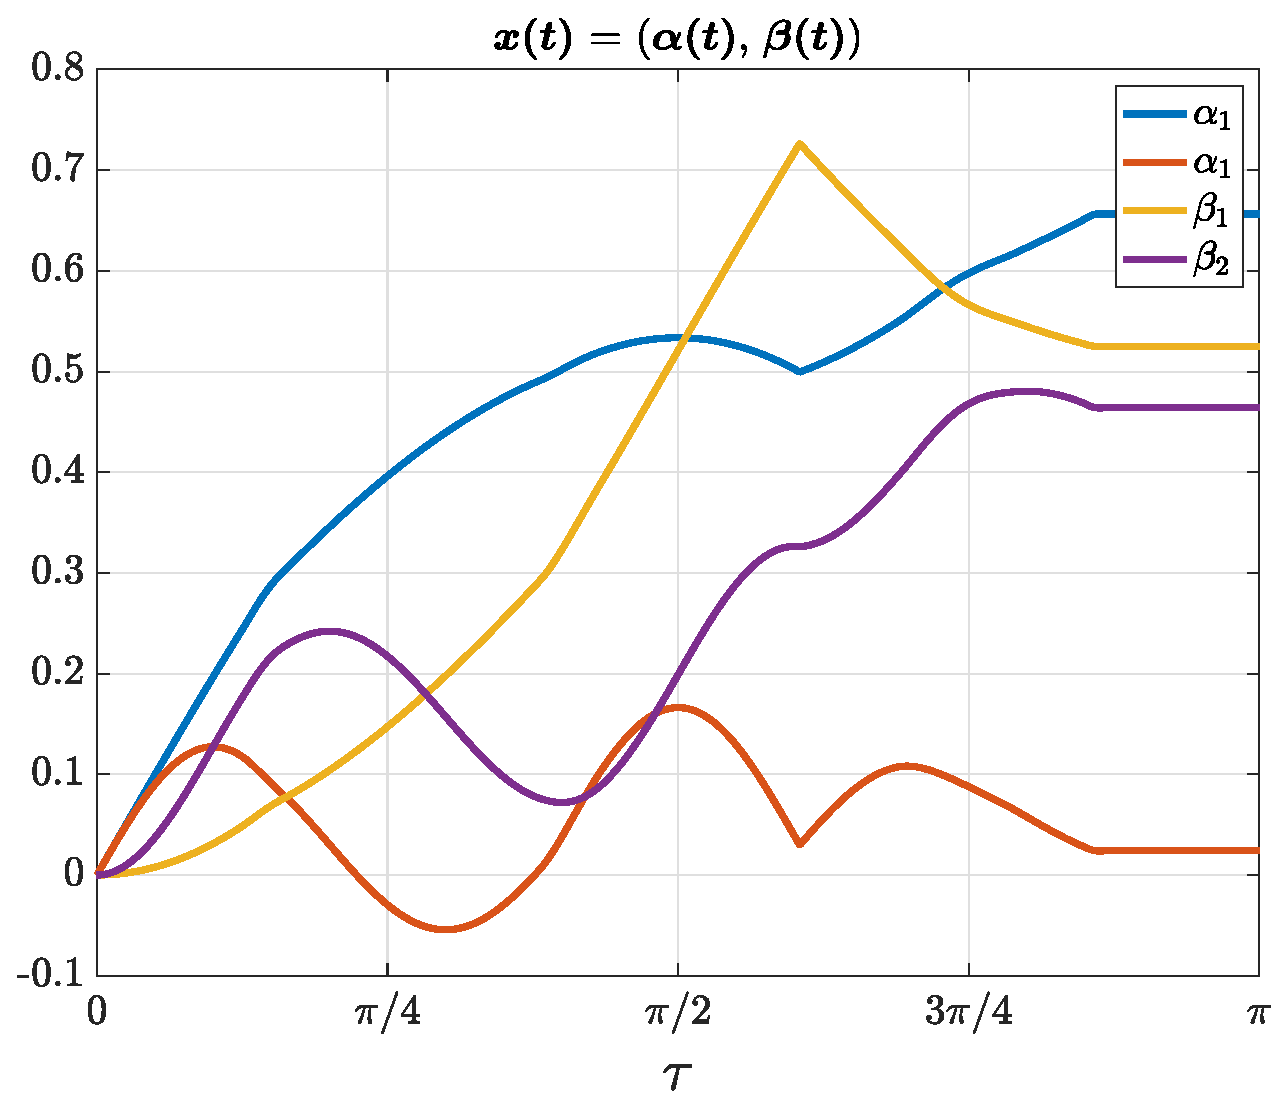
\includegraphics[scale=0.325]{img/fig02.eps}
    \caption{Evolution of the dynamical system \eqref{eq:CauchyReversed} with $\mathcal{E}_a = \{1,2\}$ and $\mathcal{E}_b = \{1,2\}$ corresponding to the control $u$ in Figure \ref{fig:exampleSHE}. The positions of the switching angles $\bm{\phi}$ are displayed as well.}\label{fig:evolution_x}
\end{figure}

A natural approach for controllability problems such as Problem \ref{pb:SHEpControl} is to formulate them as an optimal control one, where the cost functional to be minimized is the euclidean distance from the final state $\bm{x}(\pi)$ to the target, in this case, the origin. In what follows, for a given vector $\bm{v}\in\mathbb{R}^d$, we shall always denote by $\|\bm{v}\|$ the euclidean norm $\|\bm{v}\|_{\mathbb{R}^d}$.
\newline

\begin{problem}[OCP for SHM]\label{pb:OCP1}
Let $\mathcal{U}$ be a given set as in \eqref{eq:Udef} and let $\mathcal{E}_a $ and $\mathcal{E} _b $ be two finite sets of odd numbers of cardinality $|\mathcal{E}_a| = N_a $ and $ |\mathcal{E} _b| = N_b$ respectively. For any two given vectors $\bm{a}_T \in \mathbb{R}^{N_a}$ and $\bm{b}_T \in \mathbb{R}^{N_b} $, we look for an admissible control $u\in \mathcal{U}_{ad}$ solution to the following optimal control problem:
\begin{equation*}
	\min_{u \in \mathcal{U}_{ad}}\;\frac 12 \|\bm{x}(\pi)\|^2 \quad \text{subject to the dynamics \eqref{eq:CauchyReversed}},
\end{equation*}
where the set of admissible controls $\mathcal{U}_{ad}$ is defined as
\begin{align*}
	\mathcal{U}_{ad} := \{ u&\in L^\infty ([0,\pi); [-1,1]) 
	\\ 
	&\text{of the from \eqref{eq:uExpl}} \text{satisfying \eqref{eq:staircase prop}} \}.
\end{align*}
\end{problem}

\UB{I think this remark has to be either rewritten or even eliminated}

\JO{Esto viene a cuento, ya que de en el problema de optimización de SHE clasico \ref{pb:SHE opt} ocurre lo mismo.} \\


\begin{remark}
Note that, due to the coercivity of the cost functional, Problem \ref{pb:OCP1} admits at least one solution for any target $[\bm{a}_T;\bm{b}_T]^\top$. However, we say that the SHM problem admits a solution if and only if the minimum in Problem \ref{pb:OCP1} is equal to zero. Otherwise, we say that the target $[\bm{a}_T;\bm{b}_T]^\top$ is unreachable. In this work, we will not discuss the reachable set for the control problem \eqref{pb:OCP1}.
\end{remark}

Due to the constraints in the definition of the set of admissible controls $\mathcal{U}_{ad}$,  it is difficult to construct solutions to Problem \ref{pb:OCP1}. The classical tools in optimal control theory seem not to be adapted to handle such constraints on the control. In order to bypass this difficulty, we propose a modification of the optimal control problem by adding, to the cost functional, a penalization term for the control. As we shall prove, a suitable choice of this penalization term makes the optimal control have the desired staircase structure \eqref{eq:uExpl} with \eqref{eq:staircase prop}, even if we do not explicitly impose this structure as a constraint on the control. Moreover, by multiplying the penalization term by a (small) weighting parameter $\varepsilon$, we can control the precision of the optimal control for the perturbed problem, guaranteeing that the final state of the optimal trajectory is close enough to zero.

\bigskip

\begin{problem}[Penalized OCP for SHM]\label{pb:OCP_penalizado}
Fix $\varepsilon>0$ and a function $\mathcal{L}\in C([-1,1];\mathbb{R})$.  Let $\mathcal{E} _a $ and $\mathcal{E} _b $ be two finite sets of odd numbers of cardinality $|\mathcal{E}_a| = N_a $ and $ |\mathcal{E} _b| = N_b$ respectively. For any two given vectors $\bm{a}_T \in \mathbb{R}^{N_a}$ and $\bm{b}_T \in \mathbb{R}^{N_b} $, we look for a control $u\in L^\infty$ solution to the following optimal control problem:
\begin{align*}
	&\displaystyle\min_{u \in L^\infty}\;\dfrac{1}{2} \|\bm{x}(\pi)\|^2 + \varepsilon \displaystyle\int_0^\pi \mathcal{L}(u(\tau)) d\tau 
	\\[5pt] 
	&\text{subject to the dynamics \eqref{eq:CauchyReversed}},
\end{align*}
where, in this case, the set of admissible controls is just 
\begin{align*}
	L^\infty:=L^\infty ([0,\pi]; [-1,1]).
\end{align*}
\end{problem}

Observe that, in Problem \ref{pb:OCP_penalizado}, we do not impose the constraint that the control has to be the form \eqref{eq:uExpl} and satisfy the staircase property. However, for a given finite set $\mathcal{U}$ as in \eqref{eq:Udef}, we need to construct $\mathcal{L}$ in such a way that any optimal control $u^\ast$, solution to Problem \ref{pb:OCP_penalizado}, has the from \eqref{eq:uExpl}.

Another important aspect that needs to be taken into account is that the penalization term for the control might prevent the optimal trajectory from reaching the target. In other words, even if there exists a control for which the optimal trajectory satisfies $\bm{x} (\pi) = 0$, the optimal control in Problem \ref{pb:OCP_penalizado} might not do so, and therefore, the solution to Problem \ref{pb:OCP_penalizado} would not be a solution to the SHM problem. Nevertheless, by taking $\varepsilon$ small enough, we can guarantee some accuracy for the solution of Problem \ref{pb:OCP_penalizado}. This is the content of the following Proposition.

\bigskip

\begin{proposition}\label{Prop:approx controllability}
Assume that $[\bm{a}_T,\bm{b}_T]^\top$ is such that Problem \ref{pb:SHEpControl} admits a solution, and let $u^\ast\in L^\infty$ be the solution to Problem \ref{pb:OCP_penalizado}. Then the associated trajectory $\bm{x}^\ast\in C([0,\pi];\mathbb{R})$, solution to \eqref{eq:CauchyReversed}, satisfies
\begin{align*} 
	\| \bm{x}^\ast (\pi)  \|^2 \leq  4 \varepsilon \pi \| \mathcal{L}\|_\infty,
\end{align*}
where $\| \mathcal{L}\|_\infty$ denotes the max-norm in $C([-1,1]; \mathbb{R})$.
\end{proposition}

The elementary proof is postponed to Section \ref{sec:Proof}. Let us now describe the construction of penalization functions $\mathcal{L}$ which guarantee that any solution to Problem \ref{pb:OCP_penalizado} has the form \eqref{eq:uExpl} and satisfies \eqref{eq:staircase prop}. We distinguish two cases, depending on the cardinality of $\mathcal{U}$.

\subsection{Bilevel SHM problem via OCP (Bang-Bang Control)} 

In this case, the control set $\mathcal{U}$ defined in \eqref{eq:Udef} has only two elements, i.e.  $\mathcal{U}=\{-1,1\}$.
In the control theory literature, a control taking only two values is known as \emph{bang-bang control}. In the SHM literature, this kind of solution are called bi-level solutions. Note that in this case, any $u$ with the form \eqref{eq:uExpl}  trivially satisfies the staircase property \eqref{eq:staircase prop}.

\bigskip

\begin{theorem}\label{th:bang-bang}
Let $\mathcal{U}=\{ -1, 1\}$, and consider Problem \ref{pb:OCP_penalizado}. If the function $\mathcal{L}\in C([-1,1];\mathbb{R})$ is concave, then any optimal control $u^\ast$, solution to Problem \ref{pb:OCP_penalizado}, has a bang-bang structure, i.e. it has the form \eqref{eq:uExpl}.
\end{theorem}

The proof is postponed to Section \ref{sec:Proof}, and follows from the optimality conditions given by the Pontryagin's maximum principle. The fact that the control $u$ acts linearly in \eqref{eq:CauchyReversed}, together with the concavity of $\mathcal{L}$, implies that the Hamiltonian is also concave, and then, the minimum is always attained at the limits of the interval $[-1,1]$.

We point out that, by choosing different penalization functions $\mathcal{L}$, we can obtain solutions to the SHE problem with different waveforms.
Typical choices of penalization functions $\mathcal{L}$, which give rise to bang-bang controls are 
\begin{align*}
	\mathcal{L}(u) = u,  \quad \mathcal{L}(u) = -u,  \quad \mathcal{L}(u) = -u^2.
\end{align*} 
See Figure \ref{fig:Bang-Bang-penalization} for an illustration.

\subsection{Multilevel SHE problem via OCP}

Inspired by the ideas of the previous subsection, we can address the case when $\mathcal{U}$ contains more than two elements. \UB{This is known in the electrical engineering literature as the \textit{multilevel SHM problem}}. Now, the goal is to construct a function $\mathcal{L}$ such that the Hamiltonian associated to Problem \ref{pb:OCP_penalizado} always attains the minimum at points in $\mathcal{U}$.
A way to construct such a function $\mathcal{L}$ is to interpolate a parabola in $[-1,1]$ by affine functions, considering the elements in $\mathcal{U}$ as the interpolating points.  Since, between any two points in $\mathcal{U}$,  the function $\mathcal{L}$ is a straight line,  the Hamiltonian is a concave function in these intervals, and hence, the minimum is always attained at points in $\mathcal{U}$.

\vspace{1em}
\begin{theorem}\label{th:PLP}
Let $\mathcal{U}$ be a given set as in \eqref{eq:Udef}.
For some $0<a\in\mathbb{R}$ and $b\in \mathbb{R}$, set the function
\begin{align*}
	\mathcal{P}(u) = a (u-b)^2.
\end{align*}
Consider the Problem \ref{pb:OCP_penalizado} with $\mathcal{L}$ given by
\begin{align}\label{eq:PLP}
	&\mathcal{L}(u) = \begin{cases}
            \lambda_k(u) & \text{if }  u \in [u_k,u_{k+1}[ \\ \mathcal{P}(1) & \text{if } u = u_{L} 
    \end{cases} 
	\\[10pt]
	&\notag \forall k \in \{1,\dots,L-1\} 
\end{align}
where 
\begin{align}\label{eq:lambda k}
	\lambda_k(u) = \dfrac{ (u-u_k)\mathcal{P}(u_{k+1}) + (u_{k+1}- u) \mathcal{P}(u_k)}{u_{k+1} - u_k}.
\end{align}
Then any optimal control $u^\ast$, solution to Problem \ref{pb:OCP_penalizado}, has the form \eqref{eq:uExpl} and satisfies \eqref{eq:staircase prop}.
\end{theorem}

\bigskip

\begin{remark}[\emph{Bang-off-bang control}]
We note, as a special case, that when  $\mathcal{U}= \{-1,0,1\}$, we can just use the $L^1$-norm of the control as penalization function, i.e. $\mathcal{L}(u) = |u|$. This gives yields to the so-called \emph{bang-off-bang} controls, that are widely studied in the literature \cite{Wang2020}. By taking a different parabola $\mathcal{P}$, one can obtain different bang-off-bang solutions to the SHE problem.
\end{remark}

We illustrate in Figure \ref{fig:SHE-multi} different examples of penalization functions $\mathcal{L}$ giving rise to multilevel solutions to the SHE problem. We point out that, by varying the values of $a$ and $b$ in Theorem \ref{th:PLP}, we an obtain solutions with different waveforms.

\begin{remark}

We shall remark that in Theorem \ref{th:PLP} the Lagrangian $\mathcal L$ can actually have a more general form than \eqref{eq:PLP}, still yielding to an optimal control $u^\ast$, solution to Problem \ref{pb:OCP_penalizado}, with the has the form \eqref{eq:uExpl} and satisfying \eqref{eq:staircase prop}.

At this regard, assume that the finite set $\mathcal{U}$ defined in \eqref{eq:Udef} is composed by elements in ascending order. Let $\mathcal{Y} = \{y_\ell\}_{\ell=1}^L$ be another finite set, with the same cardinality as $\mathcal U$, such that the $L-1$ tuple
\begin{align*}
	\frac{\Delta \mathcal{Y}}{\Delta \mathcal{U}} = \Bigg( \frac{y_\ell - y_{\ell+1}}{u_\ell - u_{\ell+1}} \Bigg)_{\ell=1}^{L-1}
\end{align*}
is monotone. Let $\mathcal{L}:\mathbb{R} \rightarrow \mathbb{R}$ be a piece-wise continuous function:
\begin{align*}
	&\mathcal{L}(u) = \begin{cases}
		\lambda_k(u) & \text{if }  u \in [u_k,u_{k+1}[ \\ 1 & \text{if } u = u_{N_u} 
    \end{cases} 
	\\[10pt]
	&\forall k \in \{1,\dots,N_u-1\}
\end{align*}    
such that $\{y_l = \mathcal{L}(u_l)\}_{l=1}^L$. 

Then, a sufficient condition for having controls in the desired form for the SHM problem is that, for all $k \in \{1,\dots,N_u-1\}$, the functions $\lambda_k$ are concave.

Examples of functions which are compatible with this situation are
\begin{enumerate}
    \item[1.] A union of concave functions (see the second plot in Figure \ref{fig:SHE-multi}):
    \begin{align*}
        \lambda_k^{p_2}(u) = -4u^2 + 2(u_k + u_{k+1}) - 2u_{k}
    \end{align*}
    \item[2.] Linear approximation of shifted parabola (see the third plot in Figure \ref{fig:SHE-multi})
    \begin{align*}
        \lambda_k^{p_3}(u) = \frac 1 4[(u_{k+1}+u_{k}) (u-u_k-1) + u_k^2]
    \end{align*}
\end{enumerate}

\section{Numerical simulations}\label{sec:Simulations}

In this section, we present several examples in which we solve our optimal control problem through the direct method and the non-linear constrained optimization tool \texttt{CasADi} \cite{Andersson2019}. All the simulations we are going to present can be found also in \footnote{\href{https://github.com/djoroya/SHE-Optimal-Control-paper}{https://github.com/djoroya/SHE-Optimal-Control-paper}}
%
\subsection{Smooth approximation of piece-wise linear penalization}

With the final aim of using an optimization software to solve our optimal control problem, we will approximate our piece-wise linear penalization with the help of the Heaviside function $h:\mathbb{R} \rightarrow \mathbb{R}$ and its smooth approximation defined as follows: 
\begin{align*}
    h(x) = \begin{cases}
        1 & \text{ if } x \geq 0 \\ 0 & \text{ if } x < 0
    \end{cases}    
    \hspace{2em} 
    \begin{cases}
        \displaystyle h^\eta(x) = \frac 12\big(1 + \tanh(\eta x)\big) \\[7pt] \displaystyle \lim_{\eta\to\infty} h^\eta = h.
    \end{cases}
\end{align*}
Using $h$, we can define the (smooth) function $\Pi_{a,b}^\eta:\mathbb{R} \rightarrow \mathbb{R}$ as:
\begin{align*}
    \Pi_{[a,b]}^\eta(x) &= - 1 + h^\eta(x-a) + h^\eta(-x+b) 
    \\[5pt]
    &= \frac{\tanh[\eta( x -a)] + \tanh[\eta (b-x)]}{2}.
\end{align*}
In this way, we can define the smooth version of \eqref{eq:PLP}:
\begin{align*}
    \mathcal{L}^\eta(u) = \sum_{k = 1}^{N_u-1} \big[ (u_{k+1}+u_{k}) (u-u_k) + u_k^2 \big] \Pi^\eta_{[u_k,u_{k+1}]}(u).
\end{align*}
So that, when $\eta \rightarrow \infty$, then $\mathcal{L}^\eta \rightarrow \mathcal{L}$. 

\subsection{Direct method  for  OCP-SHE}

To solve the optimal control problem (\ref{pb:OCP_penalizado}), we use a direct method. 
%
If we consider a partition $\mathcal{P} = \{\tau_0,\tau_1,\dots,\tau_{T}\}$ of interval $[0,T]$ , we can represent a function $\{ u(\tau) \ | \ \tau \in [0,T]\}$ as a vector $\bm{u} \in \mathbb{R}^{T}$ where component $u_t = u(\tau_t)$.  
%
Then the optimal control problem (\ref{pb:OCP1}) can be written as optimization problem with variable $\bm{u} \in \mathbb{R}^{T}$. This problem is a nonlinear programming, for this we use CasADi software to solve. 
%
Hence, given a partition of the interval $[0,\pi)$, we can formulate the problem \ref{pb:OCP_penalizado} as the following one in discrete time
\newline

\begin{problem}[Numerical OCP]\label{pb:numOCP2}
Given two sets of odd numbers $\mathcal{E}_a$ and $\mathcal{E}_b$ with cardinalities $|\mathcal{E}_a| = N_a$ and $|\mathcal{E}_b| = N_b$ respectively, given the target vectors $\bm{a}_T  \in \mathbb{R}^{N_a}$, so that $\bm{x}_0 = [\bm{a}_T,\bm{b}_T]^\top$ and $\bm{b}_T \in \mathbb{R}^{N_b}$ and a partition $\mathcal{P}_\tau = \{\tau_0,\tau_1,\dots,\tau_{T}\}$ of the interval $[0,\pi)$, we search a vector $\bm{u} \in \mathbb{R}^{T}$ that solves the following minimization problem:
\begin{align*}
	&\min_{\bm{u} \in \mathbb{R}^T} \Bigg[\| \bm{x}^T\|^2 + \varepsilon \sum_{t=0}^{T-1} \bigg[\frac{\mathcal{L}^\eta(u_{t}) + \mathcal{L}^\eta(u_{t+1})}{2}\Delta\tau_t \bigg]  \Bigg]  
	\\[15pt]
    &\notag \text{subject to: } 
    \\
    &\forall \tau \in \mathcal{P} \begin{cases}
    \bm{x}^{t+1} = \bm{x}^{t} - (2/\pi)\Delta \tau_t \bm{\mathcal{D}}(\tau_t)u_t 
    \\
    \bm{x}^0 = \bm{x}_0
    \end{cases} 
\end{align*}
\end{problem}

\subsection{Examples}

All the examples that we are going to present will share the following common parameter: $\varepsilon = 10^{-5}$, $\eta = 10^{-5}$ and $\mathcal{P}_t = \{0.0 , 0.1, 0.2 ,\dots,\pi\}$. Moreover, we will consider $\mathcal{E}_a = \{1,5,7\}$ and  $\mathcal{E}_b = \{1,5,7\}$, and the target vectors $\bm{a}_T = (i_d,0,0)^T$ and $\bm{b}_T = (i_d,0,0)^T$ for all $i_d \in [-0.8,0.8]$. We will treat all the cases specific types of controls we mentioned before, that is, \emph{bang-bang}, \emph{bang-off-bang} and \textit{multilevel}. 

\vspace{1em}
\begin{simulation}[Bang-Bang]\label{simu1}
We consider Problem \ref{pb:numOCP2} with a set of admissible controls:
\begin{align*}
    \mathcal{U} = \{-1,1\}
\end{align*}
\end{simulation}
In accordance with Theorem \ref{th:bang-bang}, we can see in Figure \ref{fig:sim-bang-bang} how for all $i_a \in [-0.8,0.8]$ the optimal control only takes the values $\{-1,1\}$ displayed in the plot in blue and red, respectively.

\begin{figure}[ht!]
    \hspace{0.05em}
    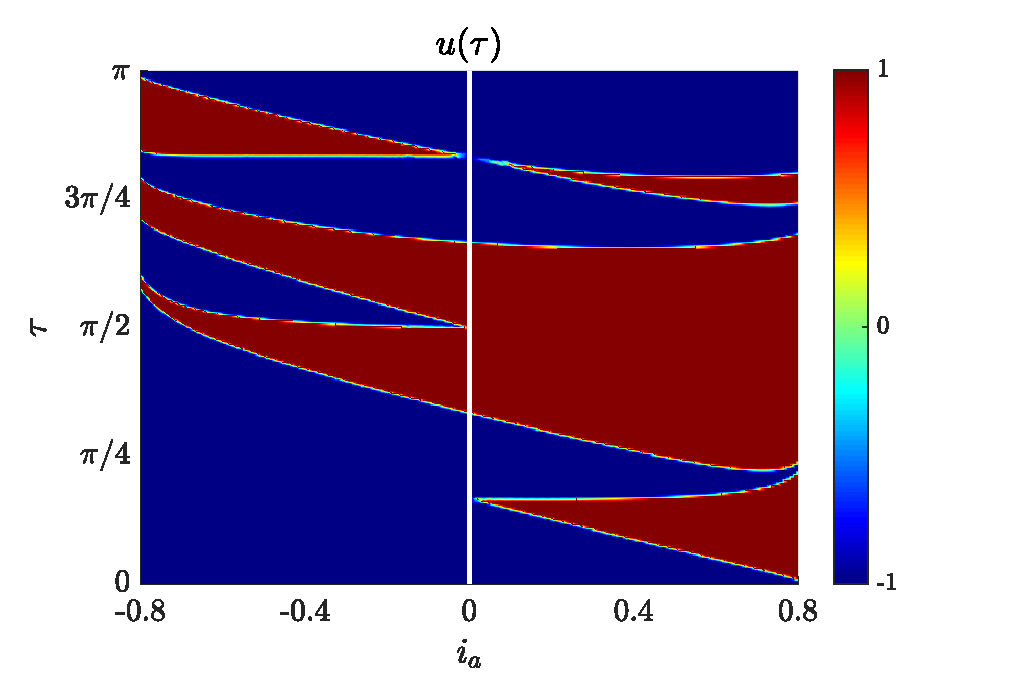
\includegraphics[scale=0.525]{img/fig05.eps}
    \caption{Results of simulation of Simulation \ref{simu1}.}\label{fig:sim-bang-bang}
\end{figure} 

\vspace{1em}
\begin{simulation}[Bang-off-Bang]\label{simu2}
We consider Problem \ref{pb:numOCP2} with a set of admissible controls:
\begin{align*}
	\mathcal{U} = \{-1,0,1\}
\end{align*}
\end{simulation}
In the same way as before, when we consider three possible values $\mathcal U = \{-1,0,1\}$, we recover the \emph{bang-off-bang} controls (Figure \ref{fig:sim-bang-off-bang}).

\begin{figure}[ht!]
    \hspace{0.05em}
    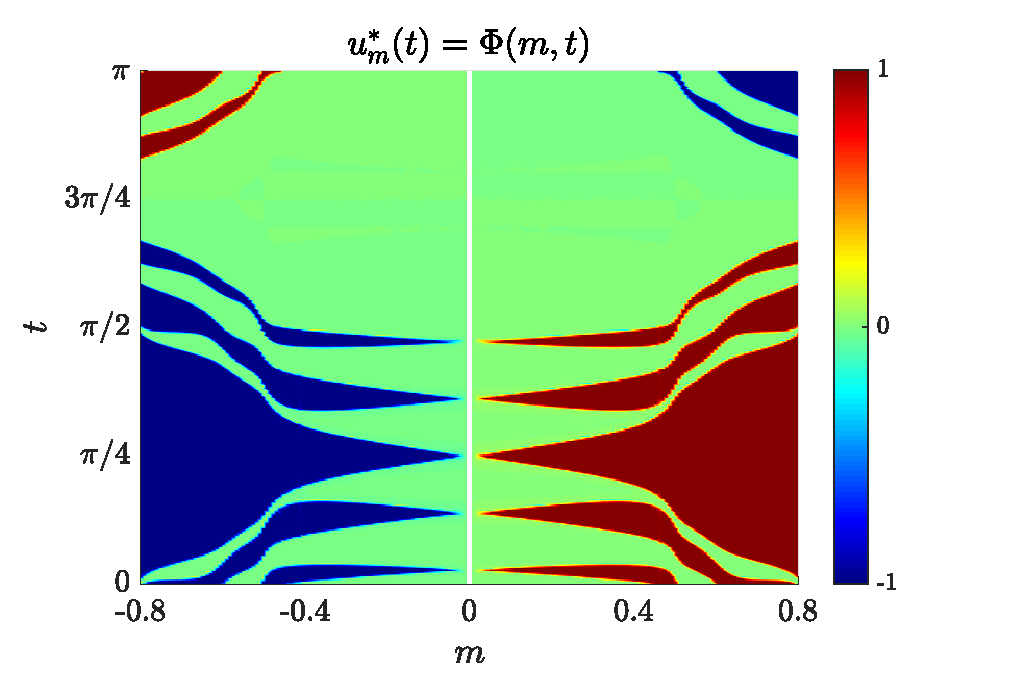
\includegraphics[scale=0.525]{img/fig06.eps}
    \caption{Results of simulation of Simulation \ref{simu2}.}\label{fig:sim-bang-off-bang}
\end{figure} 

\vspace{1em}
\begin{simulation}[Multi-level]\label{simu3}
We consider Problem \ref{pb:numOCP2} with a set of admissible controls:
\begin{align*}
    \mathcal{U} = \{-1,-1/2,0,1/2,1\}
\end{align*} 
\end{simulation}

\begin{figure}[ht!]
    \hspace{0.05em}
    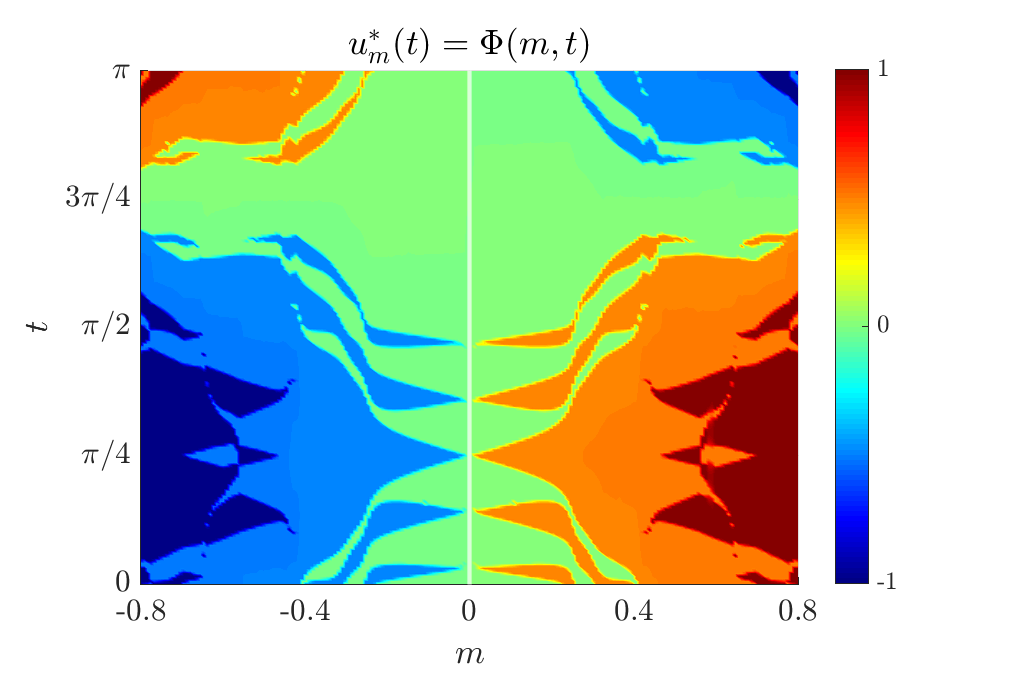
\includegraphics[scale=0.525]{img/fig08.eps}
    \caption{Results of simulation of Simulation \ref{simu3}.}
    \label{fig:sim-multi-level}
\end{figure} 

Finally, we can see in Figure \ref{fig:sim-multi-level} the same behavior when considering el mismo comportamiento cuando consideramos de el conjunto de controles admisibles $\mathcal{U} = \{-1,1\}$.
 
This methodology allows obtaining a $10^{-4}-10^{-5}$ precision in the distance to the target vector

\section{Proofs of results in Section \ref{sec:Contributions}}\label{sec:Proof}

In this section, we give the proofs of the results presented in Section \ref{sec:Contributions}. We start with the proof of Proposition \ref{Prop:approx controllability}, which gives an upper estimate for the error in the solution to the optimal control problem with the penalization term for the control. 

\bigskip

\begin{proof}[of Proposition \ref{Prop:approx controllability}]
Since we are supposing that Problem \ref{pb:SHEpControl} has a solution, there exists a control $\tilde{u}\in L^\infty((0,\pi); [-1,1])$ such that its corresponding trajectory $\tilde{\bm{x}}$, solution to \eqref{eq:CauchyReversed}, satisfies $\tilde{\bm{x}}(\pi) = 0$. 

Now, let $u^\ast$ be the solution to Problem \ref{pb:OCP_penalizado}, and let $\bm{x}^\ast$ be its corresponding trajectory. By the optimality of $u^\ast$ we have
\begin{align*}
	\frac{1}{2} \| \bm{x}^\ast(\pi)\|^2 +\varepsilon \int_0^\pi \mathcal{L}(u^\ast(\tau))d\tau \leq \varepsilon \int_0^\pi \mathcal{L}(\tilde{u}(\tau))d\tau,
\end{align*}
and hence, we deduce that $\| \bm{x}^\ast (\pi)\|^2 \leq 4 \varepsilon \pi \| \mathcal{L}\|_\infty.$ \hfill $\square$
\end{proof}

\subsection{Proofs of Theorems \ref{th:bang-bang} and \ref{th:PLP}}

The proofs of Theorems \ref{th:bang-bang} and \ref{th:bang-bang} are based on the optimality conditions for the Optimal Control Problem \ref{pb:OCP_penalizado}, which can be deduced by means of Pontryagin's maximum principle \cite[Chapter~2.7]{bryson1975applied}.

\subsubsection{Optimality conditions}

First of all, let us introduce the Hamiltonian function associated to the Optimal Control Problem \ref{pb:OCP_penalizado}:
\begin{align}\label{eq:hamil}
    \mathcal{H}(u,\bm{p},t) = \varepsilon \mathcal{L}(u) - \frac 2\pi\big(\bm{p} \cdot \bm{\mathcal{D}}(t)\big)u(t),
\end{align}
where $\bm{p}\in \mathbb{R}^{N_a+N_b}$ is the so-called adjoint variable, which arises from the restriction imposed by the dynamical system \eqref{eq:CauchyReversed}. Note that the adjoint variable $\bm{p}$ has the same dimension of the state $\bm{x}$. In view of the definition of $\bm{\mathcal{D}}(t)$ in \eqref{eq:Dynamics}-\eqref{eq:DalphaDbeta}, we will sometimes write the state and the adjoint variables using the following notation:
\begin{align*}
  \bm{x}(t) = \begin{bmatrix} \bm{a}(t) \\ \bm{b}(t) \end{bmatrix} \quad \text{and}\quad
  \bm{p}(t) = \begin{bmatrix} \bm{p}^a(t) \\ \bm{p}^b(t) \end{bmatrix}.
\end{align*}

Now, let us derive the optimality conditions arising from Pontryagin's principle.
\begin{itemize}
	\item[1.] \textbf{The adjoint system}: for any optimal control $u^\ast \in L^\infty$, solution to the Problem \ref{pb:OCP_penalizado}, there exists a unique adjoint trajectory $\bm{p}^\ast\in C([0,\pi]; \mathbb{R}^{N_a+N_b})$ which satisfies the following terminal-value problem
    \begin{equation*}
    	\begin{cases}
    		\dot{\bm{p}^\ast}(t) = -\nabla_x \mathcal{H}(u(t),\bm{p}^\ast(t),t), \qquad t \in [0,\pi] 
    		\\[5pt]
    		\bm{p}^\ast (\pi) = \nabla_x \Psi (\bm{x}^\ast (\pi))
    	\end{cases}
    \end{equation*}
    where $\Psi$ is the terminal cost of the Optimal Control Problem \ref{pb:OCP_penalizado}. In our case, we have $\Psi (\bm{x}) = \frac{1}{2} \| \bm{x}\|^2$. Moreover, since the Hamiltonian does not depend on the state variable $\bm{x}$, we simply have $\dot{\bm{p}^\ast}(t) = 0$ for all $t \in [0,\pi]$. We therefore deduce that the adjoint trajectory is constant, and given by
    \begin{equation}\label{eq:adjoint constant}
		\bm{p}^\ast (t) = \bm{x}^\ast (\pi), \qquad \forall t \in [0,\pi]. 
	\end{equation}
    
    \item[2.] \textbf{The Optimal  Control}: now, using the optimal adjoint trajectory, we can deduce the necessary optimality condition for the control, which reads as follows:
    \begin{align}\label{eq:control design}
    	u^* (t) \in \argmin_{|u|\leq 1} \mathcal{H}(t,\bm{p}^*(t),u), \quad \forall t \in [0,\pi].
    \end{align}
    As we will see, for penalization functions $\mathcal{L}$ as the ones we consider in Theorems \ref{th:bang-bang} and \ref{th:PLP}, this argmin is a singleton for almost every $t\in [0,\pi]$, and hence, given the adjoint $\bm{p}^\ast$,  condition \eqref{eq:control design} uniquely determines the control as a function in $L^\infty((0,\pi);[-1,1])$.
\end{itemize}
    
In view of \eqref{eq:hamil} and \eqref{eq:adjoint constant}, we can write the optimality condition \eqref{eq:control design} as
\begin{align}\label{eq:control design2}
    u^\ast(t)  \in & \argmin_{|u|\leq 1}  \mathcal{H}_\mu (u,\mu^\ast(t))  
    \\[5pt]
    &:=\argmin_{|u|\leq 1}   \left[\varepsilon \mathcal{L}(u) - \mu^\ast(t) u \right] \nonumber
\end{align}    
where 
\begin{align}\label{eq:m ast}
    \mu^\ast (t) := & \frac 2\pi \big(\bm{x}^*(\pi) \cdot \bm{\mathcal{D}}(t)\big) 
    \\[5pt]
    = & \sum_{i \in \mathcal{E}_a} a^*_i (\pi) \cos(it) + \sum_{j \in \mathcal{E}_b} b^*_j (\pi) \sin(jt). \nonumber
\end{align}


\subsection{Proof of Theorem \ref{th:bang-bang}}\label{proof:bang-bang}

We need to prove that, if $\mathcal{L}$ is a concave function, then any optimal control $u^\ast$ has the form \eqref{eq:uExpl} with $\mathcal{U}=\{-1,1\}$. It then suffices to prove that the argmin in \eqref{eq:control design} is the singleton $\{-1\}$ or $\{1\}$ for all $t\in [0,\pi]$ except for a finite set of $t$.

Since $\mathcal{L}$ is a concave function, so is $\mathcal{H}_\mu(u,\mu)$ as a function of $u$. Hence, in view of \eqref{eq:control design2}, we have
\begin{align*} 
	u^\ast (t)= -1  \quad \text{whenever} \; \mathcal{H}_\mu(-1,\mu^\ast(t)) <  \mathcal{H}_\mu(1,\mu^\ast(t)) 
\end{align*} 
and
\begin{align*}
	u^\ast (t)= 1  \quad \text{whenever} \; \mathcal{H}_\mu(1,\mu^\ast(t)) <  \mathcal{H}_\mu(-1,\mu^\ast(t)) .
\end{align*}
Now, in view of the definition of $\mathcal{H}_\mu$ in \eqref{eq:control design2}, we see that $u^\ast(t)$ is uniquely determined, and belongs to $\mathcal{U}$, for all $t\in [0,\pi]$ except when
\begin{align*}
	\mu^\ast (t) = \varepsilon \frac{\mathcal{L}(1) - \mathcal{L}(-1)}{2}.
\end{align*}
Finally, in view of the form of $\mu^\ast$ in \eqref{eq:m ast}, it is clear that the above equality can only hold a finite number of times in $[0,\pi]$. Indeed, the times $t\in [0,\pi]$ such that it holds are precisely the switching angles. \hfill $\square$

\begin{figure}[h] 
	\centering
	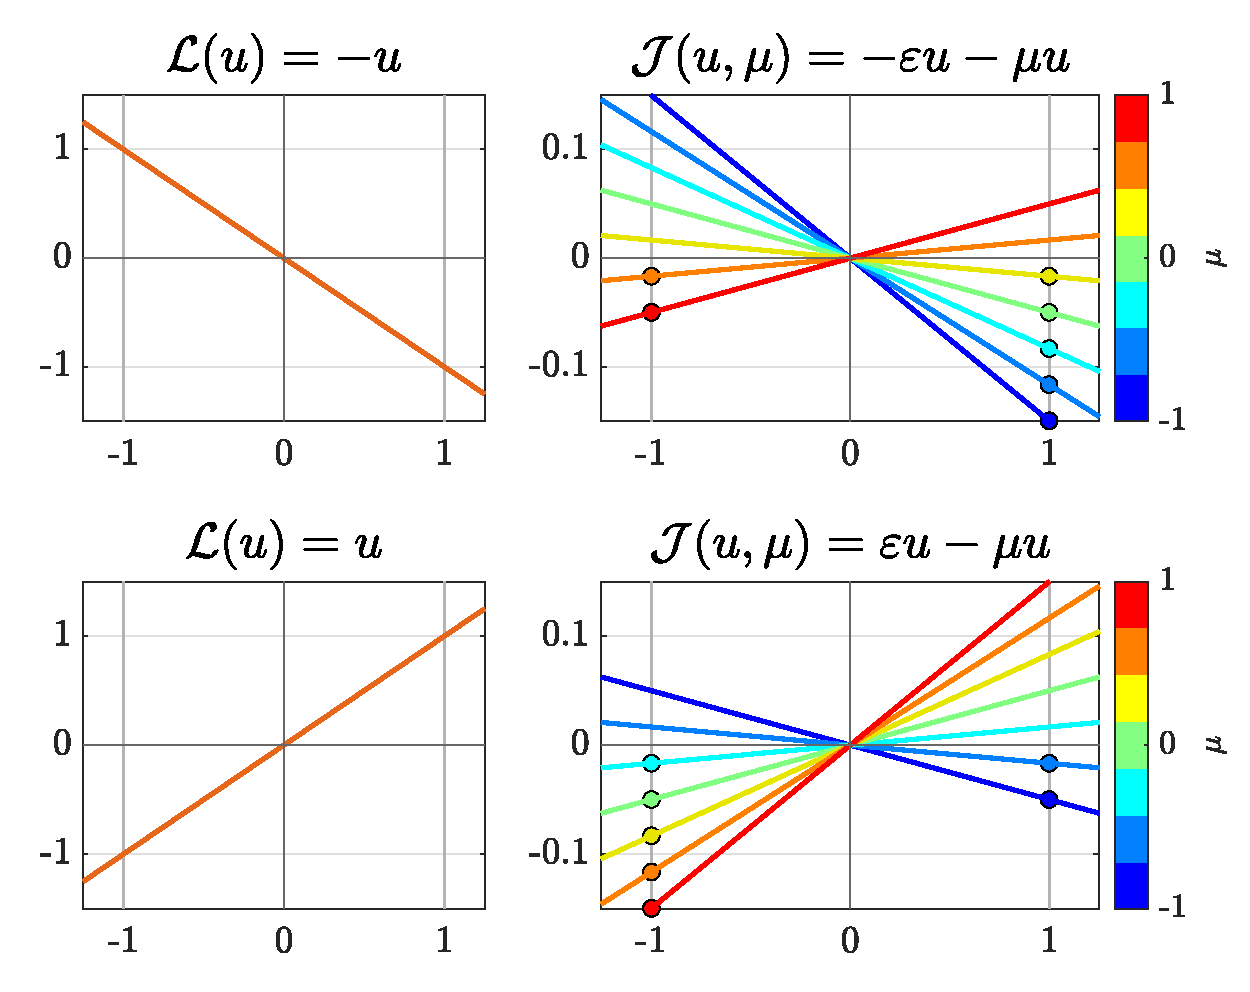
\includegraphics[scale=0.415]{img/fig03.eps}
	\caption{Bi-level SHE: in the left column we show three types of concave penalization compatibles with Theorem \ref{th:bang-bang}. In the right columns we display the behavior of the corresponding Hamiltonian for different values of $\mu$.}\label{fig:Bang-Bang-penalization}
\end{figure}

\subsection{Proof of Theorem \ref{th:PLP}}\label{proof:PLP}

In this case, we suppose that the control set $\mathcal{U} = \{ u_i\}_{i=1}^L$ is a finite set of real numbers in $[-1,1]$ satisfying
\begin{align*} 
	-1 = u_1 < u_2 <\ldots <u_L = 1, \quad \text{with} \ L> 2.
\end{align*} 
The case $L=2$ is just the bi-level case. As in the previous proof, we only need to prove that the argmin in \eqref{eq:control design2} is a singleton and belongs to $\mathcal{U}$ for every $t\in [0,\pi]$ except for a finite number of times $t\in [0,\pi]$.

In this case, the study of the minimizers of $\mathcal{H}_\mu$ is a bit more involved since the penalization function $\mathcal{L}$ defined in \eqref{eq:PLP}-\eqref{eq:lambda k} is not differentiable. However, $\mathcal{L}$ is an affine interpolation of a convex function, so it is Lipschitz and convex.  Hence, $\mathcal{H}_\mu$ is also Lipschitz and convex as a function of $u$. We can therefore use the following necessary and sufficient condition for $u$ to be a minimizer of  the function 
\begin{align*}
	u\mapsto \mathcal{H}_\mu (u,\mu)
\end{align*}
if and only if
\begin{equation}\label{opti cond subdiff}
	0\in \partial_u \mathcal{H}_\mu (u,\mu),
\end{equation}
where $\partial_u$ denotes the subdifferential with respect to $u$. Let us recall the definition of subdifferential from convex analysis:
\begin{align*}
	\partial_u \mathcal{H}_\mu (u,\mu) = \{  & c\in \mathbb{R} \quad \text{s.t.} 
	\\
	&\mathcal{H}_\mu (v,\mu) - \mathcal{H}_\mu (u,\mu) \geq c(v-u) 
	\\
	& \forall v\in [-1,1] \}. 
\end{align*}
In the case of a convex function, one may show that the subdifferential at $u\in (-1,1)$ is the nonempty interval $[a,b]$, where $a$ and $b$ are the one-sided derivatives
\begin{align*}
	a &= \lim_{v\to u^-} \frac{\mathcal{H}_\mu (v,\mu) - \mathcal{H}_\mu(u,\mu)}{v-u} 
	\\[5pt]
	b &= \lim_{v\to u^+} \frac{\mathcal{H}_\mu (v,\mu) - \mathcal{H}_\mu(u,\mu)}{v-u}. 
\end{align*}
Moreover, the subdifferential at $u=-1$ and $u=1$ are given by $(-\infty, b]$ and $[a,+\infty)$ respectively.

Using this characterization of the subdifferential, we can compute $\partial_u\mathcal{H}_\mu(u,\mu)$ for all $u\in [-1,1]$ in terms of $\mu$.
Let us define
\begin{align*} 
	p_k := \frac{\mathcal{P}(u_{k+1}) - \mathcal{P} (u_k) }{u_{k+1} - u_k} 
\end{align*} 
for all $k\in \{1, \ldots, L-1\}$. Now, using the definition of $\mathcal{H}_\mu$ in \eqref{eq:control design2} and $\mathcal{L}$ in \eqref{eq:PLP}, we can compute
\begin{align*}
	&\partial_u \mathcal{H}_\mu (-1,\mu) = (-\infty, \varepsilon p_1 -\mu], 
	\\[5pt]
	&\partial_u \mathcal{H}_\mu (1,\mu) = [\varepsilon p_{L-1} -\mu, +\infty), 
	\\[5pt]
	&\partial_u \mathcal{H}_\mu (u_k,\mu) = [\varepsilon p_{k-1} -\mu,  \, \varepsilon p_k -\mu],
\end{align*}
for all $k\in \{ 2, \ldots, L-1\}$, and
\begin{equation*}
	\partial_u \mathcal{H}_\mu(u,\mu) = \{\varepsilon p_k -\mu\},
\end{equation*}
for all $u\in (u_k, u_{k+1})$ and all $k\in \{ 1, \ldots, L-1 \}$.

Now we observe that
\begin{equation}\label{eq:subdiff}
	\begin{array}{ll}
		0\in \partial_u \mathcal{H}_\mu (-1,\mu) & \quad\text{iff}\quad  \mu\leq  \varepsilon p_1, 
		\\[5pt]
		0\in \partial_u \mathcal{H}_\mu (1,\mu) & \quad\text{iff} \quad \mu\geq  \varepsilon p_{L-1}, 
		\\[5pt]
		0\in \partial_u \mathcal{H}_\mu (u_k,\mu) & \quad\text{iff} \quad  \varepsilon p_{k-1} \leq \mu \leq \varepsilon p_k , 
	\end{array} 
\end{equation}
for all $k\in \{ 2, \ldots, L-1\}$,  and, for all $k\in \{ 1, \ldots, L-1 \}$,
\begin{equation*}
	0\in \partial_u \mathcal{H}_\mu (u,\mu) \quad \text{for all}\  u\in [u_k, u_{k+1}]
\end{equation*}
if and only if $\mu= \varepsilon p_k$.

Using this, along with the optimality condition \eqref{opti cond subdiff}, we deduce that, for almost every $\mu\in \mathbb{R}$, we have
\begin{align*}
	\argmin_{u\leq 1} \mathcal{H}_\mu (u,\mu) = \{u_k\}
\end{align*}
for some $u_k\in \mathcal{U}$. Indeed, \eqref{opti cond subdiff} does not hold if and only if $\mu= \varepsilon p_k$, for some $k\in \{1,\ldots, L-1\}$.

Hence, using the optimality condition for $u^\ast(t)$ in \eqref{eq:control design2}, we see that $u^\ast(t)$ is uniquely determined, and belongs to $\mathcal{U}$, for all $t\in [0,\pi]$ except when
\begin{align*}
	\mu^\ast(t) = \varepsilon \frac{\mathcal{P}(u_{k+1}) - \mathcal{P}(u_k)}{u_{k+1} -u_k}
\end{align*} 
for some $k\in\{1,\ldots, L-1\}$. In view of the form of $\mu^\ast(t)$ in \eqref{eq:m ast}, it is clear that the above equality can only hold a finite number of times in the interval $[0,\pi]$. Indeed, we refer to the set of times when the above equality holds as the switching angles.
Due to the continuity of $\mu^\ast(t)$, along with \eqref{eq:subdiff}, it is clear that $u^\ast(t)$ does not change value between two consecutive switching angles. The staircase property of the waveform \eqref{eq:staircase prop} can also be deduced from \eqref{eq:control design2} and \eqref{eq:subdiff}, along with the continuity of the function $\mu^\ast(t)$.\hfill $\square$

\begin{figure}[h]
	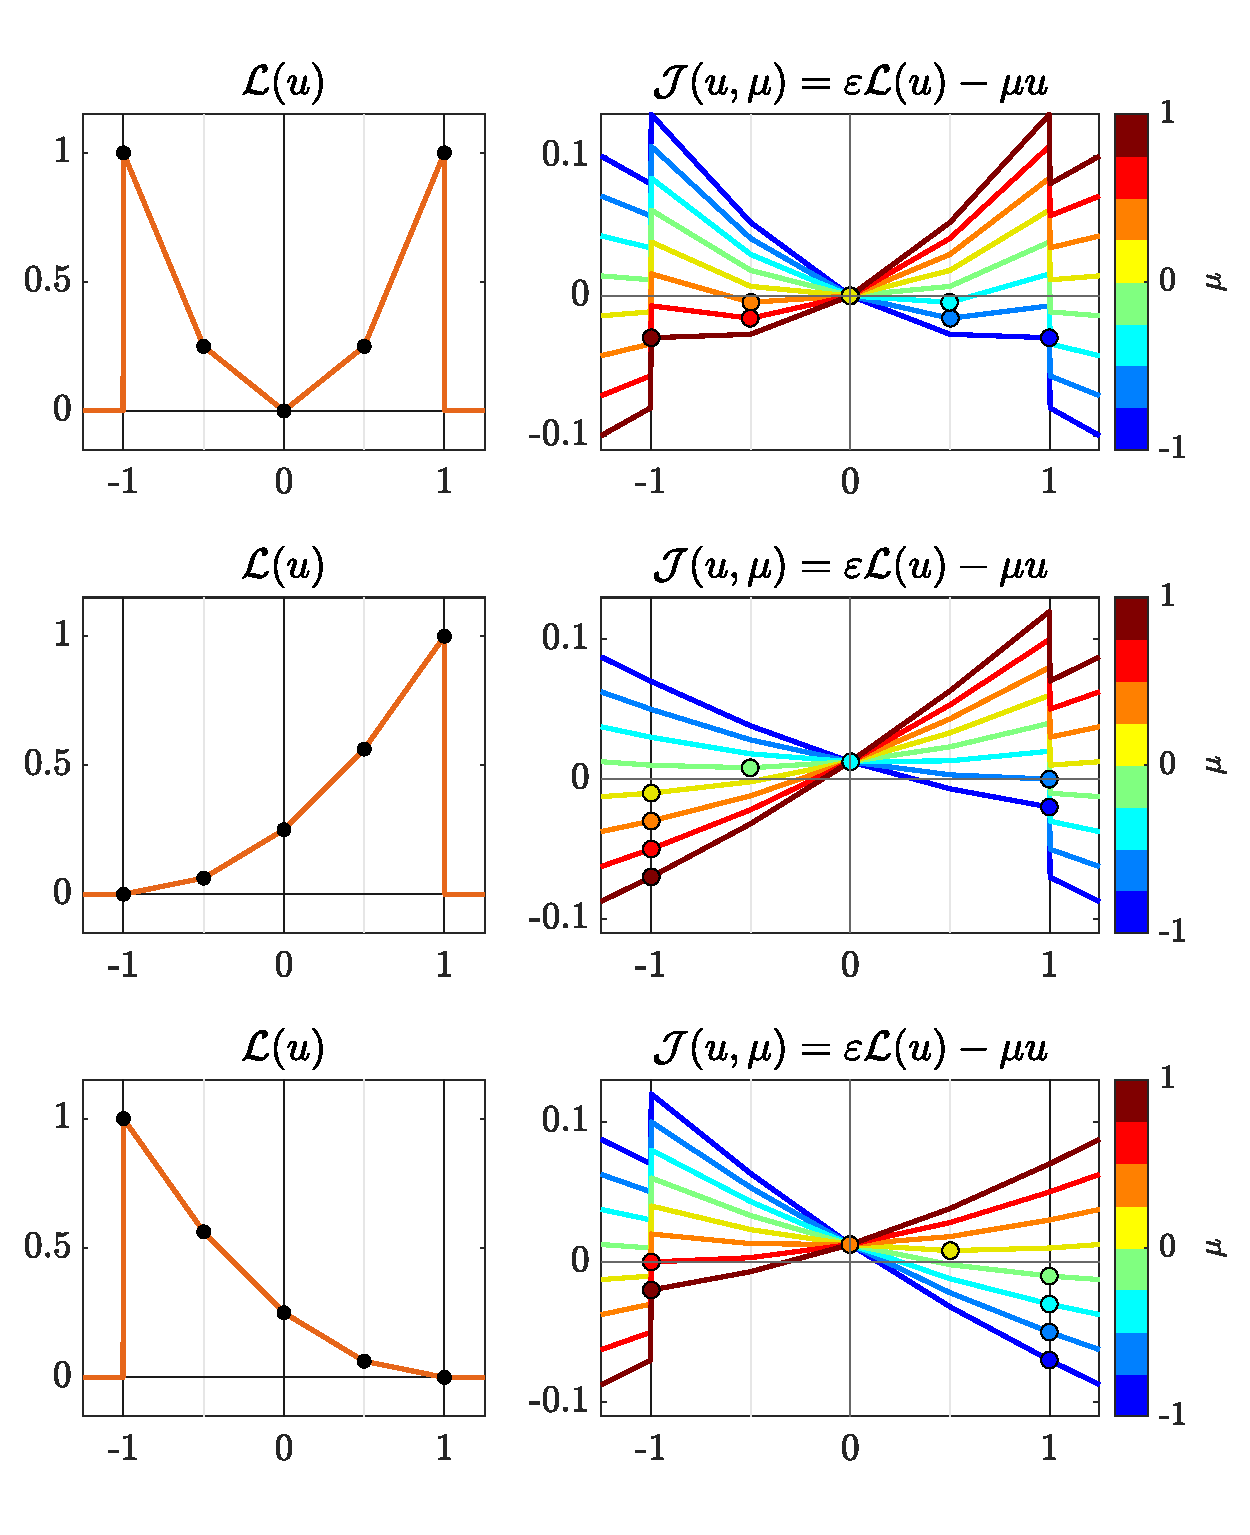
\includegraphics[scale=0.415]{img/fig04.eps}
	\caption{Multilevel SHM: in the left column we show three types of penalizations which are compatible with our theoretical results. In the right column we show the behavior of the corresponding Hamiltonian for different values of $\mu$.}\label{fig:SHE-multi}
\end{figure} 
\end{remark}



%Hence, we have $\partial H_m = \varepsilon\partial \mathcal{L} - m$. This means that, given $m\in \mathbb{R}$, we look for $u \in [-1,1]$ minimizing $\mathcal{H}_m(u)$. It is then necessary to determine whether zero belongs to $\partial \mathcal{H}_m(u)$.
%
%\begin{itemize}
%    \item \textbf{Case 1: $m \leq \varepsilon(u_1+u_2)$}: since $m$ is less than the  minimum of all subdifferentials, then zero does not belong to any of the intervals we defined. Hence, the minimum is in one of the extrema
%    \begin{gather}
%        \argmin_{|u| < 1} \mathcal{H}_m(u) = u_1
%    \end{gather} 
%    \item \textbf{Case 2: $m = \varepsilon(u_{k+1}+u_k) $}: taking into account that $\forall k \in \{1,\dots,N_u-1\}$,
%    \begin{gather}
%        \argmin_{|u| < 1} \mathcal{H}_m(u) = [u_k,u_{k+1}[ 
%    \end{gather} 
%    \item \textbf{Case 3: $\varepsilon(u_k+u_{k-1})<m<\varepsilon(u_{k+1}+u_k)$}: taking into account that $\forall k \in \{2,\dots,N_u-1\}$,
%    \begin{gather}
%        \argmin_{|u| < 1} \mathcal{H}_m(u) = u_k
%    \end{gather}
%    \item \textbf{Case 4: $m>\varepsilon(u_{N_u}+u_{N_u-1})$}:
%    \begin{gather}
%        \argmin_{|u| < 1} \mathcal{H}_m(u) = u_{N_u}
%    \end{gather} 
%\end{itemize}
%
%In other words, only when $m = \varepsilon(u_{k+1}+u_k)$ the minima of the Hamiltonian belong to an interval. For all the other values of $m\in\mathbb{R}$, these minima are contained in $\mathcal{U}$. So that under a continuous variation of $m$, Case 2 can only occur pointwise. Recalling the optimal control problem $m(\tau) = [\bm{p}(\tau) \cdot \bm{\mathcal{D}}(\tau)]$, we can notice that Case 2 corresponds to the instants $\tau$ of change of value.






\section{Conclusiones}\label{Section6}


We presented the SHE problem from the point of view of control theory. Nevertheless, comparing with methodologies where the commutation number is fixed a priori, our approximation is computationally more expensive. Notwithstanding that, the optimal control provides solutions in the entire range of the modulation index, although the number of solutions or their locations change dramatically.

This methodology for the SHE problem connects control theory with harmonic elimination. In this way, the SHE problem can be solved through classical tools.


\subsection{Quarter wave symetry}
We shall mention that, in the SHE literature \cite{Wu2009}, it is usual to distinguish among the half-wave symmetry problem (addressed in the present paper) and the quarter-wave symmetry one in which
    \begin{align*}
        u\left(\tau + \frac \pi2\right) = -u(\tau)\quad \mbox{for all}\; \tau \in \left[0,\frac \pi2\right).
    \end{align*}
    In quarter-wave symmetry, the SHE problem simplifies, as the Fourier coefficients $\{a_i\}_{i\in\mathcal E_a}$ turn out to be all zero. Hence, only the phases of the converter's signal can be controlled, while the half-wave SHE allows to deal with the amplitudes as well. It is worth to remark nonetheless that our optimal control formulation can be easily adapted to the quarter-wave symmetry problem by simply replacing the Fourier coefficients \eqref{eq:an} with
    \begin{align*}
        a_i = 0, \quad\quad b_j = \frac{4}{\pi} \int_0^{\frac \pi4} u(\tau)  \sin(j \tau)\,d\tau.
    \end{align*}
    Entonces podemos introducir el siguiente sistema dinámico:
    \begin{gather}
        \begin{cases}
            \displaystyle \dot{\bm{\beta}}(\tau) = \frac 2\pi \bm{\mathcal{D}}^\beta(\tau) u(\tau), & \tau \in [0,\pi/2)
            \\[6pt]
            \bm{\beta}(0) = \bm{b}_T
        \end{cases}\label{eq:CauchyReversed_4sym}
    \end{gather}
    Además del siguiente problema de control:
    \vspace{0.5em}
    \begin{problem}\label{pb:SHEpControl_4sym}
        Let $\mathcal{U}$ be defined as in \eqref{eq:Udef} and let $\mathcal{E} _b $ be a set of odd numbers with cardinality $ |\mathcal{E} _b| = N_b$. Given the vector $\bm{b}_T \in \mathbb{R}^{N_b} $. We look for $u:\in [0,\pi/2)\to\mathcal{U}$ such that the solution of \eqref{eq:CauchyReversed_4sym} with initial datum $\bm{x}(0)=\bm{x}_0$ satisfies $\bm{x}(\pi)=0$.
    \end{problem}
    Donde de la misma forma que en el problema con simetría de media onda la solución de este problema es también solución del problema SHE con simetría de cuarto de onda.

\subsection{Generalizations}


Consideramos que el tipo de penalizaciones utilizados en este problema puedes ser extendido a sistemas LTI:
\begin{gather}
	\min_{u \in \mathcal{U}}\;\frac 12 \|\bm{x}(T)\|^2 + \int_0^T \mathcal{L}(u(\tau))d\tau
	\\
    \notag \text{subject to: }\quad \begin{cases}
            \displaystyle \dot{\bm{x}}(\tau) = A(\tau)x(\tau) +B(\tau)u(\tau),  & \tau \in [0,T)\\[6pt]
            \bm{x}(0) = \bm{x}_0
    \end{cases}
\end{gather}

De manera que dado un término de penalización compatible con el Teorema \ref{th:GeneralP}, sea capaz de condicionar el control óptimo como un control digital.


\begin{ack}            
This project has received funding from the European Research Council (ERC) under the European Union’s Horizon 2020 research and innovation programme (grant agreement NO: 694126-DyCon). The work of U.B. and J.O. is partially supported by the Elkartek grant KK-2020/00091 CONVADP of the Basque government. The work of U.B. is partially supported by the Air Force Office of Scientific Research (AFOSR) under Award NO: FA9550-18-1-0242 and by the Grant MTM2017-92996-C2-1-R COSNET of MINECO (Spain).
\end{ack}
 
\bibliographystyle{apalike}        % Include this if you use bibtex 
\bibliography{bib}           % and a bib file to produce the 
                                 % bibliography (preferred). The
                                 % correct style is generated by
                                 % Elsevier at the time of printing.


 

\end{document} 